%\documentcrass{svjour3}                     % onecolumn (standard format)
%\documentclass[smallcondensed]{svjour3}     % onecolumn (ditto)
\documentclass[smallextended]{svjour3}       % onecolumn (second format)
%\documentclass[twocolumn]{svjour3}          % twocolumn

\smartqed  % flush right qed marks, e.g. at end of proof

% \usepackage{mathptmx}      % use Times fonts if available on your TeX system

% insert here the call for the packages your document requires
\usepackage[utf8]{inputenc}
% Use nameref to cite supporting information files (see Supporting Information section for more info)
\usepackage{nameref,hyperref}
% amsmath and amssymb packages, useful for mathematical formulas and symbols
\usepackage{amsmath,amssymb}
% useful for consistent display and control of units of measurement
\usepackage{siunitx}
% figures!
\usepackage{graphicx}
% for including TODO notes
\usepackage{todonotes}
% syntax highlighting for code
\usepackage{minted}
% Uncomment next two lines to add line numbers.
\usepackage{lineno}
\linenumbers

\journalname{Sports Engineering}

\begin{document}

\title{Analysis and Ethical Design of Terrain Park Jumps for Snow Sports}

\author{
  Jason~K. Moore \and
  Bryn Cloud \and
  Mont Hubbard \and
  Christopher~A. Brown
}

%\authorrunning{Short form of author list} % if too long for running head
\institute{
  J.~K. Moore \at
  Delft University of Technology\\
  Mekelweg 2, 2628 CD Delft, The Netherlands\\
  \email{j.k.moore@tudelft.nl}
  \and
  B. Cloud \& M. Hubbard \at
  University of California, Davis\\
  One Shields Ave., Davis, CA 95616 USA\\
  \email{becloud@ucdavis.edu,mhubbard@ucdavis.edu}
  \and
  C.~A. Brown \at
  Worcester Polytechnic Institute\\
  100 Institute Rd., Worcester, MA 01609 USA\\
  \email{brown@wpi.edu}
}

\date{Received: date / Accepted: date}
% The correct dates will be entered by the editor

\maketitle

\begin{abstract}
  Most American snowsport resorts now have terrain parks and decades-long
  epidemiological evidence correlates terrain park use with injuries.
  Engineering design of jumps could reduce injuries by limiting equivalent fall
  heights (EFHs), which indicate dissipated landing impact energy. No evidence
  refutes making terrain park jumps safer in this way. We discuss case studies
  illustrating that large EFHs are significant factors in traumatic injuries on
  terrain park jumps. Standards and design tools for builders can make jumps
  safer. We introduce a tool that can evaluate existing jumps as well as design
  jump profiles with safer equivalent EFHs to reduce injuries.
\end{abstract}

\section{Introduction}
\label{intro}
%
Impacts with fixed surfaces can cause injury. Greater velocities, perpendicular
to the surfaces, provide greater injury potential due to increased kinetic
energy dissipation. Equivalent fall height (EFH) is a conceptually simple and
familiar measure of impact danger used in safety standards worldwide, from
construction~\cite{OSHA2021} to children's playground
equipment~\cite{Chalmers1996}. EFHs of terrain park jumps can be calculated
using techniques in \cite{Levy2015} from Cartesian coordinates of jump
profiles. Profiles must include starting points, takeoff ramps, and landing
hills, along jumpers' paths. Controlling energy dissipation in human bodies,
hence EFH on jumps, is ethical engineering because it reduces the likelihood
and severity of injuries. EFH should be a primary attribute of jump design. It
must be considered because it is clearly connected to injury risk and can be
used to design and construct safer jumps.

Societal costs of jump injuries are discussed here with case studies that
illustrate dangers if EFH is not limited appropriately. We also discuss papers
purporting to be ski safety research, which attempt to sow doubt about EFH
relevance, written by authors that regularly provide expert testimony for
defending the ski industry in personal injury lawsuits. Proposals for improved
safety are absent in the papers. We present a user-friendly web application
that can facilitate jumping injury reduction by calculating EFH on current and
future jumps.

\subsection{History}
\label{sec:hist}
%
Terrain park jumps are not new. Gradual introduction in the 1980's was
accompanied by increased interest in aerial maneuvers and extreme sports
participation. Jumps have proliferated since and are today nearly ubiquitous.
Roughly 95\% of US ski resorts include terrain parks. Unfortunately, this
growth correlates with injuries. Two early longitudinal studies in the 1980's
and early 1990's~\cite{Deibert1998,Furrer1995} already found significant
increases in head injuries and concussions. Between 1993 and 1997 head injuries
accompanied most skiing and snowboarding deaths~\cite{CPSC1999}. Koehle et
al.~\cite{Koehle2002} stated ``[S]eventy-seven percent of spinal
injuries~\cite{Tarazi1999} and 30\% of head injuries~\cite{Fukuda2001} in
snowboarding were a result of jumps.'' Jackson et al.~\cite{Jackson2004}
determined that by 2004 snow skiing replaced football as the second leading
cause of serious head and spinal cord injuries in America.

These early increasing injury assessments persisted. According to
\cite{Russell2014}, ``between 5\% and 27\% of skiing and snowboarding injuries
occur[red] in terrain parks
\cite{Bridges2003,Goulet2007,Moffat2009,Greve2009,Brooks2010,Ruedl2013}''.
Incredibly, at the first Winter Youth Olympic Games more than a third of all
snowboard half-pipe and slope-style competitors were injured~\cite{Ruedl2012}.
Epidemiological research~\cite{Carus2016,Audet2020,Hosaka2020} continues to
show that injuries on terrain park jumps are more likely and more severe than
on normal slopes. Audet et.~al~\cite{Audet2020} provides evidence that skiing
or snowboarding in a terrain park is a risk factor for head, neck, back, and
other severe injuries. Hosaka et. al~\cite{Hosaka2020} concludes that jumping is a
main cause for serious spinal injuries, regardless of skill level, and suggests
that, because spinal injuries incidence  have not decreased over time,  the ski
industry should focus on designing fail-safe jump features to minimize risks of
serious spinal injuries. Similar suggestions appeared in peer-reviewed
literature for more than a
decade~\cite{Hubbard2009,Swedberg2012,McNeil2012,McNeil2012a,Hubbard2015,Levy2015,Petrone2017,Moore2018}.

\section{Equivalent Fall Height}
\label{sec:efh}
%
\emph{EFH}, a common proxy measure for impact danger in industrial safety
standards, is the weight-specific kinetic energy that must be dissipated on
falling impact from height $h$~\cite{Muller1995,Hubbard2009,Gasser2018}.
Initial potential energy $mgh$ is transformed to kinetic energy available to
injure in non-rotating falls. Injury potential can be reduced by controlling
impact circumstances, e.g. impact cushioning, and body orientation,
configuration, and motion; however this energy must still be dissipated. Larger
EFHs require more elaborate measures to reduce injury; reducing EFH does not.

EFH can be interpreted by the general public. People have an intuitive danger
sense when faced with potential falls from large heights and a strong
experiential common sense for relating fall height to likelihood of injury.
People sense increasing danger associated with falling from larger heights.
Ground, second, and third floor falls are about 2.6, 5.1, 8.8~\si{\meter},
respectively~\cite{Vish2005}. The US Occupational Safety and Health
Administration requires protection for heights greater than 1.2~\si{\meter} for
general workplace safety~\cite{OSHA2021}.  Chalmers et al.~\cite{Chalmers1996}
argues for 1.5~\si{\meter} maximum fall heights for playground equipment. The
Swiss Council for Accident Prevention makes specific recommendations for EFHs
to be below 1.5~\si{\meter} for jumps requiring basic skills~\cite{Heer2019}.
Even with no standards in Olympic Nordic ski jumps, typical ``equivalent
landing height``~\cite{Gasser2018} is only about 0.5~\si{\meter}.

EFH $h$ of objects is formally defined as
%
\begin{equation}
  h = \frac{v^2}{2g}
  \label{eq:efh_general}
\end{equation}
%
where $v$ is impact velocity and $g$ gravitational acceleration.  Kinetic
energy of objects moving at  velocity $v$  is transformed from potential energy
at height $h$; indisputable, fundamental physics.

From equation~\ref{eq:efh_general} equivalent fall heights $h$ can be
determined for any surface, i.e., sloped landing profile or shape, after
jumping~\cite{Petrone2017}. The result, neglecting air drag, is
%
\begin{align}
  h = \left[\frac{x^2}{4(x\tan\theta_T - y)\cos^{2}\theta_T} - y\right]
    \sin^{2}
    \left[\tan^{-1}\left(\frac{2y}{x} - \tan\theta_T\right) -
    \tan^{-1}\frac{dy}{dx}\right]
  \label{eq:efh}
\end{align}
%
a function only of takeoff angle $\theta_T$, impact coordinates $(x,y)$
relative to takeoff, and landing surface slope $\frac{dy}{dx}$, but not a
function of takeoff speed~\cite{Petrone2017}. To analyze jumps, one measures
Cartesian coordinates of landing surfaces along jumpers' flight paths and
takeoff angles. Slopes $\frac{dy}{dx}$ are computed from measured coordinates
$(x,y)$. Curvature for the last several meters before takeoffs must be near
zero to avoid unintentional inversion, although this does not influence EFHs.

\section{Case Studies}
\label{sec:case}
%
In these American lawsuits juries ruled for injured plaintiffs. Negligent jump
design and construction contributed significantly to
injuries~\cite{SuperiorCourtSanFranciscoCounty2002,KingCountySuperiorCourt2008}.
Simulations below use methods in \cite{Levy2015}, assuming skier mass, frontal
area, and drag coefficient of 75~\si{\kg}, 0.34~\si{\meter\squared}, and 0.821,
respectively.

\subsection{Vine v. Bear Valley Ski Company}
\label{sec:vine}
%
In April 2000, Ms.~Vine's lower spine was injured when she landed badly skiing a
jump at Bear Valley in California. The jump shape
(Fig.~\ref{fig:vine-v-bear-valley}) was a common form called a ``table-top''.
Builders intend that jumpers completely clear the table, landing on down-slopes
near a ``sweet spot''.  The upper panel of Fig.~\ref{fig:vine-v-bear-valley}
shows the  measured jump surface from accident investigation. Vine landed short
of the knuckle (end of the table-top). This table-top, typically flat and
horizontal, was instead concave, compounding dangers of short landings. At the
11~\si{\meter} measured landing horizontal distance from  takeoff, the surface
sloped upwards approximately 5\si{\degree}. The concave shape emphasizes
detrimental effects of not aligning surface tangents closer to jumper flight
paths at impact.
%
\begin{figure}
  \centering
  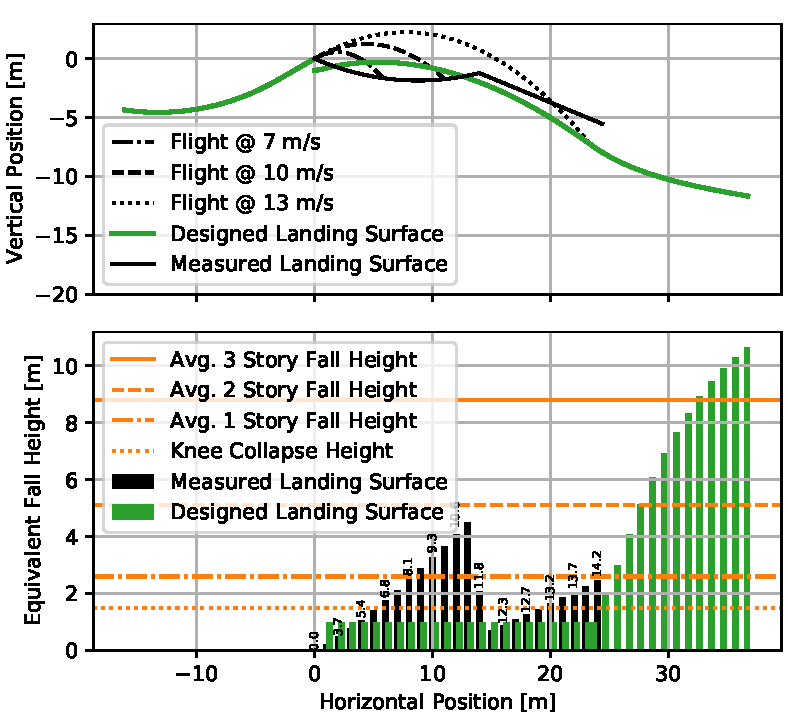
\includegraphics[width=\columnwidth]{figures/vine-v-bear-valley.pdf}
  \caption{\textbf{Bear Valley jump compared to possible safer design}
  Top: Measured landing surface (solid black) and jumper flight paths
  (intermittent black) from measured 30\si{\degree} takeoff angle.  A
  14~\si{\meter\per\second} takeoff speed is used as the design
  speed~\cite{Levy2015} for a comparison jump (solid green) shaped to have
  constant EFH of 1~\si{\meter}.
  Bottom: EFH for both jumps in corresponding colors at 2~\si{\meter}
  intervals. Numbers above bars indicate takeoff speeds required to land at
  that location.
  Intermittent horizontal gray lines indicate increasing relatable fall
  heights: knee collapse, average 1\textsuperscript{st} story fall, and average
  2\textsuperscript{nd} story fall.
  }
  \label{fig:vine-v-bear-valley}
\end{figure}

The lower panel displays EFH at different landing locations, which is greatest
just short of the knuckle.  At the sweet spot just past the knuckle the EFH
drops precipitously to  about 1~\si{\meter} but landing in this narrow region
requires jumpers to control takeoff speeds within 1~\si{\meter\per\second}.
Landing at 11 meters, Vine's EFH was almost 4 meters, equivalent to falling
from between one and two stories~\cite{Vish2005}. She had also rotated backward
in flight, landed on her lower spine and was paralyzed. A lower EFH could have
decreased likelihood of injury, due to lower impact forces.

In contrast, landing surfaces designed to have smaller EFHs can be created at
similar cost. The green jump profile in the upper panel of
Fig.~\ref{fig:vine-v-bear-valley} shows a possible jump design,
see~\cite{Levy2015}, of similar size with similar flight times that ensures a
constant (smaller) EFH of about 1~\si{\meter}. The convex shape of this jump is
interestingly close to the original concave table-top  inverted, showing that
convex landing shapes are critically important for limiting EFHs. This
alternative jump design would have lowered impact forces for landings at all
locations. In 2002, the jury ruled in favor of Ms.~Vine, agreeing that Bear
Valley was responsible for not designing safer jumps.

\subsection{Salvini v. Ski Lifts Inc.}
\label{sec:salvini}
%
In 2004, Mr.~Salvini attempted a table-top jump on skis in the terrain park of
The Summit at Snoqualmie Ski Resort, in Washington state. Salvini overshot the
intended landing location while traveling at typical skiing speeds, rotated
backward during flight and landed on his back, ultimately suffering
quadriplegia. At his landing location of 30~\si{\meter} the EFH was over 10
meters, approximately a 3-story fall.  Figure~\ref{fig:salvini-v-snoqualmie}
shows the measured jump surface from the accident investigation.  For takeoff
speeds greater than 13~\si{\meter\per\second}, the lower panel shows that the
EFH is greater than 10~\si{\meter} and grows linearly with larger takeoff
speeds. Severe injury is almost certain in falls this high, especially if
landing body orientation loads the spine, as in this case.
%
\begin{figure}
  \centering
  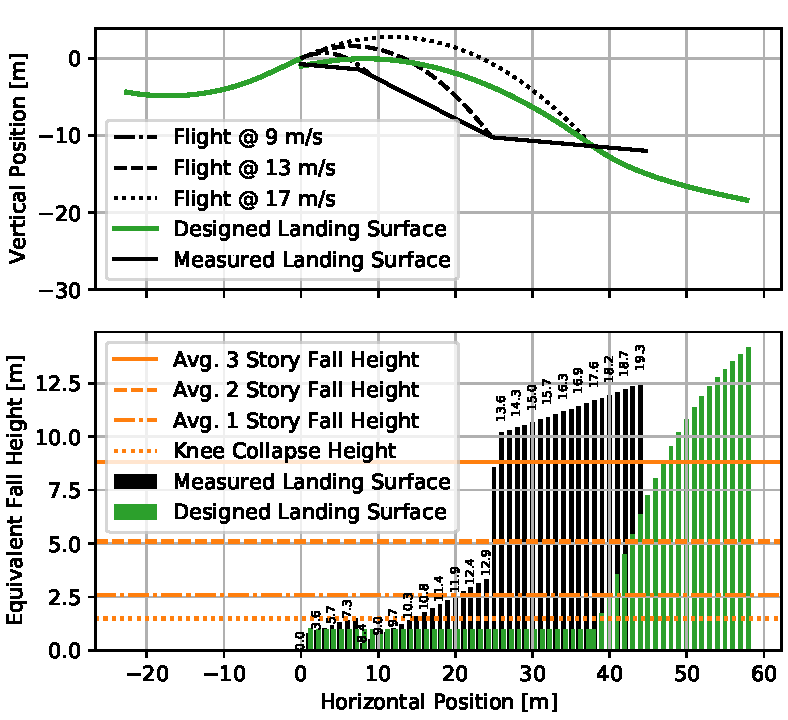
\includegraphics[width=\columnwidth]{figures/salvini-v-snoqualmie.pdf}
  \caption{\textbf{Snoqualmie jump compared to possible safer design}
  Top: Measured landing surface (solid black) and jumper flight paths
  (intermittent black) for measured 25\si{\degree} takeoff angle. The
  16~\si{\meter\per\second} takeoff speed is used as the design speed for a
  comparison jump (solid green) with constant equivalent fall height of
  1~\si{\meter}.
  Bottom: Equivalent fall height for both jumps in corresponding colors at
  2~\si{\meter} intervals. Numbers above bars indicate takeoff speed required
  to land at that location.
  Intermittent horizontal gray lines indicate increasing relatable fall
  heights: knee collapse, average 1\textsuperscript{st} story fall, average
  2\textsuperscript{nd} story fall, and average 3\textsuperscript{rd} story
  fall.
  }
  \label{fig:salvini-v-snoqualmie}
\end{figure}

The upper panel also shows a jump profile (green) designed to have a
1~\si{\meter} equivalent fall height for all speeds below
16~\si{\meter\per\second}. This profile requires significantly more snow than
the measured jump but alleviates dangerous impacts.

This jump highlights how extreme EFHs become if jumps are not properly
designed. Few recreational skiers will jump out three story windows, snow or
not. Injuries are clearly likely.  Our internal altimeter tells us so, but it's
not easy to discern when visually assessing a jump's safety.

These two case studies clearly demonstrate that deficient jump shapes have
devastating consequences and that engineering analysis and design, based on
laws of mechanics, can be used to shape jump landings that limit EFHs.
Designing jumps this way is based on well-established, centuries-old mechanics
of Newton and Émilie du Châtelet~\cite{Zinsser2007}, fundamental to physics and
engineering education. Designing jumps to limit EFHs appropriately reduces
injury risks by reducing impact energies, absolutely.

\section{Moral Imperative}
\label{sec:moral}
%
``Hold paramount the safety, health and welfare of the
public''~\cite{NSPE2019}, is the first canon of engineering ethics. The moral
imperative of engineering ethics is motivating. The first canon compels
engineers to use technical expertise to protect snowsport participants from
injuries. No one can rationally argue that reducing EFH increases likelihood of
injury. Building well designed, safe jumps is no more laborious than building
poorly designed, unsafe jumps. There is no reason not to control EFHs with good
design methods. Nonetheless skiing industries and their insurance companies are
reluctant to adopt and endorse such design methods. They hire expert witness
engineers to sow doubt on simple, basic physics, while ignoring the first
canon. Why?

In their book ``Merchants of Doubt''~\cite{Oreskes2010}, Oreskes and Conway
have studied this problem more generally. They show that in numerous industries
over the last 60 years, scientific evidence accumulated that commonly accepted
industrial activities were harmful, either to individuals or society. But the
industries had vested interests in continuing the status quo since operational
changes would have led to significant, short-term costs. Examples carefully
described and analyzed~\cite{Oreskes2010} are the use of DDT, smoking tobacco,
acid rain due to coal-fired power plants, ozone hole caused by CFCs,
second-hand tobacco smoke’s effects, and CO2-caused climate change, among
others. Rather than using the proven science as a basis for changes in
practice, strategic responses of industries have been to ``emphasize the
controversy among scientists and the need for continued
research''~\cite{Oreskes2010}.

This same strategy is used by the snowsport industry and its defense experts.
To sow doubt and counter solid, fundamental, scientific concepts of landing
hill design limiting EFH, defense experts introduce confounding factors to
cloud and confuse basic issues.  Consider three papers
\cite{Shealy2010,Shealy2015,Scher2015} co-authored by well-known skiing
industry defense experts who have testified for the snowsport resorts and their
insurance companies.

Shealy et.~al~\cite{Shealy2010} conducted an experimental study attempting to
test the hypothesis that takeoff speed is a predictor of the distance from a
jump take-off to landing. They reached the mechanically preposterous
conclusions both that there is ``no statistically significant relationship
between takeoff speed and the distance traveled'' and that ``takeoff speed is
not a dominant or controlling factor (in how far a jumper
travels)''~\cite{Shealy2010}. These conclusions were used to question the
soundness of analytical mechanical modeling of jumper flight used in
\cite{Hubbard2009,McNeil2012}.

Some of these same authors later vouched for terrain park jump safety. Using
data held by the National Ski Areas Association (NSAA), Shealy et.
al~\cite{Shealy2015} concluded that their ``hypothesis that jumping features
resulted in an increase risk of injury [was] not ...
substantiated.''~\cite{Shealy2015} This is the only study we are aware of with
this conclusion. It is difficult to reconcile it with the voluminous
contradictory research documenting the unique dangers posed by terrain park
jumps in tens of other studies cited both herein and in
\cite{Hubbard2009,Swedberg2012,McNeil2012,McNeil2012a,Hubbard2015,Levy2015,Petrone2017,Moore2018}.
Although NSAA releases yearly the total of resort-related fatalities and
catastrophic injuries, the raw data on which \cite{Shealy2015} was based is not
publicly available.

In a third experimental study (N=13) specifically designed ``to evaluate injury
mitigation potential of surfaces limiting EFH''~\cite{Scher2015}, Scher et al.
clearly show that body orientation, i.e. falling directly on one's head (in all
trials), can cause dangerous cervical spine compression loads~\cite{Scher2015},
even at low fall heights. They report on effects of EFH but only test heights
from \SIrange{0.23}{1.52}{\meter}, committing a similar fault as in
\cite{Shealy2010}, restricting ranges of their independent variables, and
ignoring fall heights known to have caused severe injuries regardless of body
orientation. Yet they insinuate that EFH has no appreciable effect on injuries.
The title, ``Terrain Park Jump Design: Would Limiting Equivalent Fall Height
Reduce Spinal Injuries?'' implies that they appear to believe that falling from
greater heights might \emph{not} cause greater injuries. Why propose such
mechanically flawed hypotheses?

Poorly executed, limited experiments, no matter how expensive the
instrumentation, cannot disprove the fundamental laws of mechanics. If
statistics or experimental results seem to conflict with predictions from
classical mechanics, the problems must be with the statistical or experimental
design or its interpretation, but not with fundamental laws of mechanics.
Defending practices that lead to injuries helps prolong these dangerous
practices, which leads to further injuries, clearly contradictory to ethical
engineering. It is difficult to get otherwise intellectually competent
engineers to appreciate the damage they do in their defense work. As Upton
Sinclair wrote ``it is difficult to get a man to understand something when his
salary depends on his not understanding it''~\cite{Sinclair1994}.

None of these papers was written to reduce injuries. No suggestions are made
how their findings can be used to promote public safety. Instead they attempt
to obscure the mechanically irrefutable fact that impacting surfaces at lower
velocities is safer. Introducing bogus science is as prevalent in American
skiing litigation defense, as it was in defending tobacco~\cite{Oreskes2010}.

American legal, healthcare and insurance systems corrupt technical literature
for legal defense of unsafe practices. Peer-reviewed technical literature is
used to support testimony in lawsuits. Both plaintiffs and defendants hire
experts, authors of technical papers, to testify.  When supporting the defense,
this can result in denying compensation for injuries and prolonging unsafe
practices. American healthcare systems can leave families of paralysis victims
destitute with little recourse but to sue snowsport resorts. American health
insurance companies also sue resorts to recover their losses in injury cases.
Conflicts of interest go undeclared in papers and presentations, for organizing
and chairing meetings, and editing publications. Financial support for
publications gets routed through consulting companies providing plausible
deniability of actual conflicts.

In injury cases, testifying for injured plaintiffs and testifying defending
insurance companies are not ethically equivalent. One attempts to address
problems that cause injuries, holding paramount the public's safety, health and
welfare. The other attempts to defend practices that might have contributed to
the injury, to limit financial losses of insurance companies. The proverbial
two sides to every question is not valid in science and engineering.

\section{What Can Be Done?}
\label{sec:action}
%
Societal needs should be addressed. Preventable injuries on terrain park jumps
should cease. Injured people require appropriate care that should not depend on
prolonged adversarial litigation clouded by deceptive engineering. Papers
helping to perpetuate dangerous practices do not belong in engineering journals
or conferences.

Everything possible should be done to eliminate dangerous jumps. Ski area
operators and their grooming staff must be educated and given tools. Standards
are needed for jump designs with limited EFHs, specifying verification,
inspection, and maintenance during use. Certification programs are needed for
jump building, inspecting, and maintenance.

As an example of a successful certification program, around 1980 ASTM Committee F27 began to develop ski binding standards.
Proponents were led by orthopedic surgeons and academic
researchers~\cite{Bahniuk1996}.  Industry argued that standards were impossible
because release value measurement was impossible by ski shops (industry now
makes similar arguments about jumps). Nevertheless certifications and
inspection standards for bindings were developed, and now there are far fewer
lower-extremity equipment-related injuries. Now in F27, no medical
professionals and almost no academics remain.

In parallel to standards development, assessing and reshaping existing jumps
eliminating dangerous EFH should be an easy route for ski resorts to increase
proactively terrain park safety. Accurate enough measurements of existing
slopes can occur with simple tools, e.g. tape measure and digital level,
consuming relatively little time per jump, see
Appendix~\ref{sec:jump-shape-measurement}. Calculation and visualization of
EFHs from these measurements can take some time without a program for
calculating EFHs from hill profiles. We have made a user-friendly,
freely-accessible online web application available with the calculation and
visualization steps almost instantaneous for jump builders. With the tool
described in the next section, jump builders can easily add this safety
assessment to their toolbox, even using it from a smartphone on hills.  We see
no reason that this basic assessment should not be part of jump construction
processes. The only ethical decision is to adopt these methods; saving even one
person from a life of paralysis, or even death, must be worth the relatively
minor inconvenience of shaping jumps using the methods in reference
\cite{Levy2015}.

\subsection{Software and Online Access}
\label{sec:software}
%
We presented the first version of software for designing ski jumps with a
specified EFH in \cite{Moore2018}. It comprises a general-purpose, extensible,
object-oriented software library with tools for 2D skiing simulation. Using
this code, a web application was developed for interactive jump design. The web
application is designed for a non-technical end-user and operable on any
desktop, tablet, or mobile device supporting a web browser.

We have extended the capabilities of the software in version 1.4.0 to assist
the work described in this paper. New library features automate calculation of
EFH for jump profiles described by a set of Cartesian coordinates.
Additionally, a new ``analysis'' page allows users to upload measured jump
profile coordinates in either a .CSV or Microsoft Excel spreadsheet file. The
jump is then analyzed and the equivalent fall height is displayed graphically
for interactive user manipulation and viewing.
Figure~\ref{fig:web-app-screenshot} shows the web application with one of the
case study jumps loaded for analysis and explains its primary features.
%
\begin{figure}
  \centering
  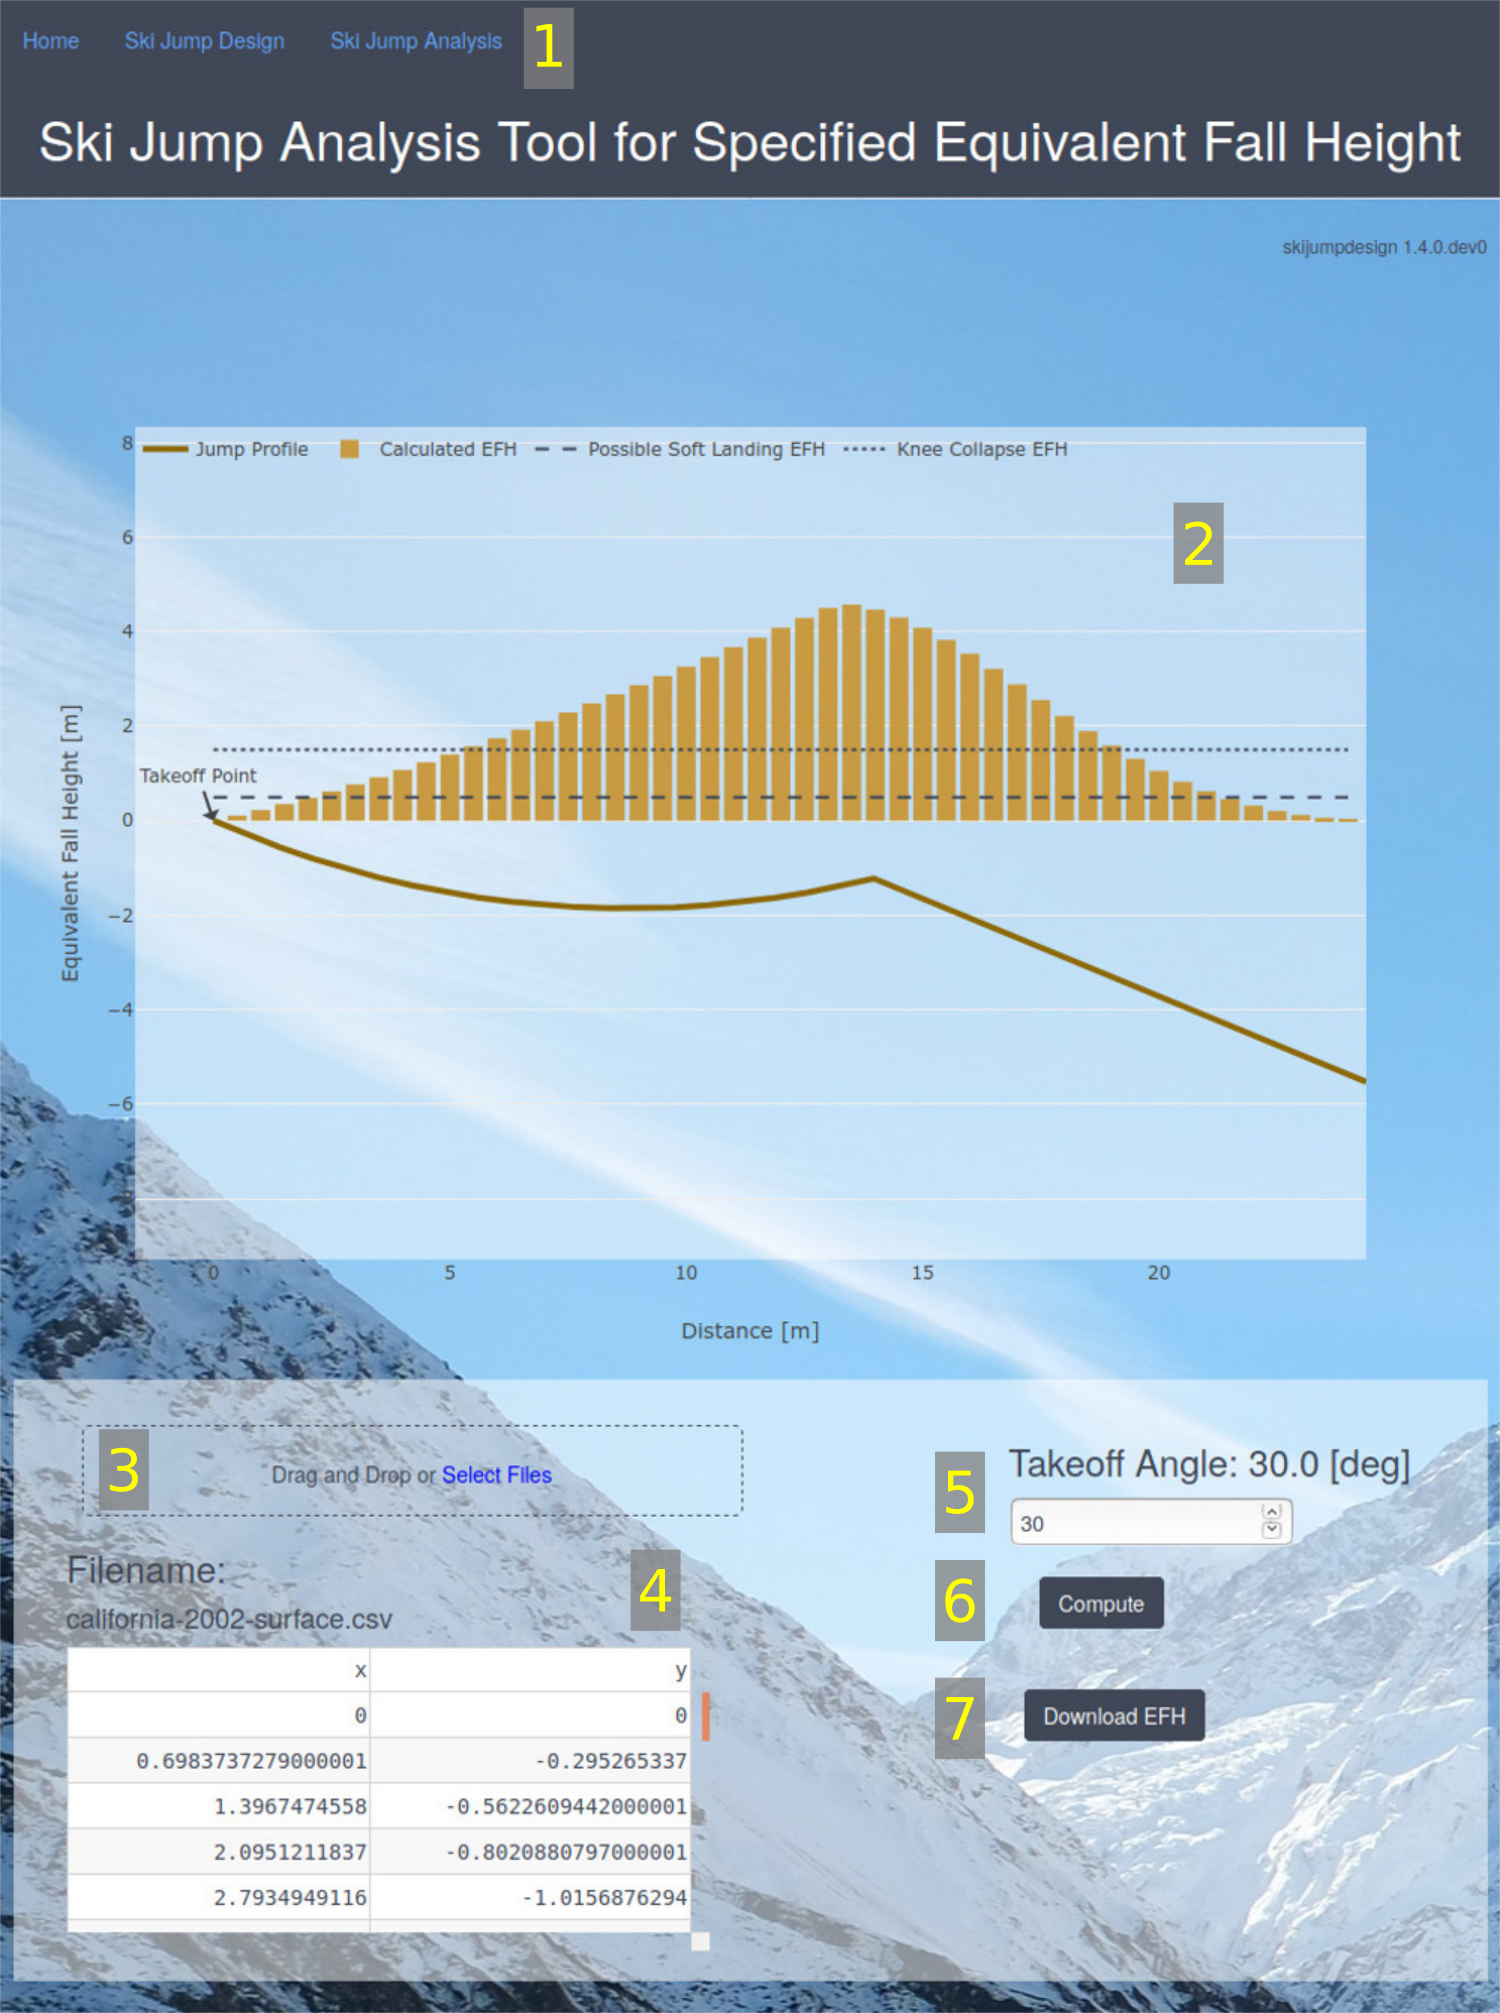
\includegraphics[width=\columnwidth]{figures/web-app-screenshot.png}
  \caption{\textbf{Screenshot of the ski jump design and analysis web app} To
    use the analysis portion of the app, a user selects ``Ski Jump Analysis''
    from the primary menu [1], uploads a .CSV or .XLS file by dragging it onto
    the screen [3], inspects the input data for accuracy in the table [4], sets
    the takeoff angle [5], runs the analysis by pressing the ``Run Analysis''
    button [6], views the results in the interactive plot [2], and downloads
    the results by pressing the ``Download EFH'' button [7].}
  \label{fig:web-app-screenshot}
\end{figure}

The software is written in Python and directly depends on popular packages
including Cython~\cite{Behnel2011}, matplotlib~\cite{Hunter2007},
NumPy~\cite{Oliphant2006}, pandas~\cite{McKinney2020}, Plotly \&
Dash~\cite{Plotly2015}, pycvodes~\cite{Dahlgren2018},
SciPy~\cite{Virtanen2020}, SymPy~\cite{Meurer2017}, and xlrd. The software is
open source and licensed under the MIT redistribution license. The source code
is distributed on PyPi (\url{https://pypi.org/project/skijumpdesign}. Users can
submit bug reports, feature requests, code improvements, and additions at the
Gitlab repository (\url{https://gitlab.com/moorepants/skijumpdesign}). The
software library is documented at \url{https://skijumpdesign.readthedocs.io}.
Basic examples of using the library are provided in the documentation and this
paper's appendix. The web app is hosted for free use at
\url{http://www.skijumpdesign.info}.

\section{Conclusion}
\label{sec:conc}
%
There are, of course, more factors than jump landing surface shape that
contribute to injuries on terrain park jumps. Yet impact velocity can be easily
controlled with a designed landing surface shape. There is no evidence that
decreasing EFH increases injuries in falls; injuries can only decrease.  Thus
there is no reason not to adopt constant low values of EFH for public-use jump
designs. Common sense is really all that is needed to believe that falling from
higher heights will increase injuries, other factors held constant.  Any person
that must fall would surely choose to do so from the lowest height.
Constructors of jumps that are not designed with these facts in mind are
negligent. The safety, health, and welfare of the public involved in this sport
should be held paramount.

\begin{acknowledgements}
  We thank Rado Dukalski for feedback on the web application and both Yumiko
  Henneberry and Lyn Taylor for feedback on the manuscript.
\end{acknowledgements}

\section*{Declarations}
\begin{description}
  \item[Funding] Not applicable
  \item[Conflict of interest] MH served as a plaintiff's expert witness in the
    two case studies discussed above. CB testifies occasionally on the side of
    plaintiffs in ski and snowboard injury cases, has collaborated with Shealy,
    and C.~D. Mote, Jr., Sher's doctoral advisor, on ski safety research, has
    participated in ASTM F27 since the 1980s on standards for bindings, boots,
    and skis, and he holds patents on ski and snow board binding designs,
    intended to reduce injuries.
  \item[Availability of data and material] All data is available at
    \url{https://gitlab.com/moorepants/skijumpdesign} and
    \url{https://gitlab.com/mechmotum/ski-jump-analysis-paper}.
  \item[Code availability] The skijumpdesign version 1.4.0 source code is
    archived at \url{https://doi.org/10.5281/zenodo.4637076}. Additionally, it
    and the paper's source code is available at
    \url{https://gitlab.com/moorepants/skijumpdesign} and
    \url{https://gitlab.com/mechmotum/ski-jump-analysis-paper}.
  \item[Author's contributions] JM and MH contributed to the study conception
    and design. Material preparation, data collection and analysis were
    performed by JM and MH. The first draft of the manuscript was written by
    JM, BC, MH, and CB. CB was primarily responsible for drafting the sections
    on ethics. All authors read and approved the final manuscript. BC and JM
    wrote the accompanying software.
  \item[Ethics approval] Not applicable
  \item[Consent for publication] JM, BC, MH, and CB consent for publication.
\end{description}

% BibTeX users please use one of
%\bibliographystyle{spbasic}      % basic style, author-year citations
% This one looks good but orders the papers by alphabetical order of last name:
%\bibliographystyle{spmpsci}      % mathematics and physical sciences
% The titles don't show up in this one:
%\bibliographystyle{spphys}       % APS-like style for physics
% None of the three supplied bib styes from Springer match Sports Engineering's guidelines. ieeetr at least orders them correctly.
\bibliographystyle{ieeetr}
\bibliography{references}   % name your BibTeX data base

\appendix

\section{Example Software Library Use}
\label{sec:example}
%
The closed form equation~\ref{eq:efh} is useful for understanding the
fundamental relationship of equivalent fall height to the landing surface
shape. It will predict EFH for small jumps but other factors may be useful to
include in the model. For example, jumpers are subject to aerodynamic drag and
this is not negligible for larger jumps. If drag is included there is no closed
form solution for the equivalent fall height, but the equivalent fall height
can be computed through iterative simulation~\cite{Levy2015}. The jumper's
flight path is found by integrating the flight equations of motion at various
takeoff velocities and computing the misalignment of jumper landing and slope
angles to then compute the equivalent fall height. This more general simulation
method is implemented in the software described herein and the results reflect
the inclusion of both gravitational and drag forces. Even with drag
incorporated, the calculating EFH still only require measurements of the
landing surface cross-sectional profile coordinates $(x,y)$ relative to the
takeoff point and a measurement of the takeoff angle.
Listing~\ref{lis:example-efh-calc} demonstrates the new software library
features creating a surface from some measured data points and then calculating
the equivalent fall height at 0.2\si{\meter} increments.
%
\begin{listing*}
  \begin{minted}{pycon}
>>> import numpy as np
>>> from skijumpdesign import Surface, Skier, plot_efh
>>> takeoff_ang = 10  # degrees
>>> takeoff_point = (0, 0)  # (x, y) in meters
>>> x_ft = np.array([-232.3,-203.7,-175.0,-146.3,-117.0,-107.4,
...    -97.7,-88.0,-78.2,-68.5,-58.8,-49.1,-39.4,-34.5,-29.7,
...    ...
...    38.8,43.3,47.8,52.3,56.8,61.5,66.2,70.9,75.7,80.6,85.5,
...    88.4,88.4])
...
>>> y_ft = np.array([55.5,46.4,37.7,29.1,22.2,19.7,17.2,14.8,
...    12.5,10.2,7.7,5.2,2.9,1.8,0.7,-0.2,-1.0,-1.2,-1.4,-1.6,
...    ...
...    -16.2,-18.1,-19.8,-21.4,-22.9,-24.0,-25.0,-25.6,-25.6])
...
>>> x_mt = x_ft*0.3048 # convert to meters
>>> y_mt = y_ft*0.3048 # convert to meters
>>> # create a surface from the data
>>> measured_surf = Surface(x_mt, y_mt)
>>> # create a skier
>>> skier = Skier(mass=75.0, area=0.34, drag_coeff=0.821)
>>> # calculate the equivalent fall height
>>> x, efh, v = measured_surf.calculate_efh(
...     np.deg2rad(takeoff_ang), takeoff_point, skier, increment=0.2)
...
>>> x  # display the x coordinates
array([ 0. ,  0.2,  0.4,  0.6,  0.8,  1. ,  1.2,  1.4,  1.6,  1.8,  2. ,
        2.2,  2.4,  2.6,  2.8,  3. ,  3.2,  3.4,  3.6,  3.8,  4. ,  4.2,
       ...
       24.2, 24.4, 24.6, 24.8, 25. , 25.2, 25.4, 25.6, 25.8, 26. , 26.2,
       26.4, 26.6, 26.8])
>>> efh  # display the equivalent fall height for each x coordinate
array([0.        , 0.02541035, 0.03479384, 0.03264587, 0.05956476,
       0.09096091, 0.12358184, 0.13702364, 0.15202999, 0.17018343,
       ...
       3.93910556, 3.97387212, 4.00891899, 4.04424779, 4.07984952,
       4.11573359, 4.68049185, 5.53413479, 6.45253722, 7.42628019])

>>> v  # display takeoff speeds to reach x positions
array([0.07373847, 0.13081777, 0.1878382 , 0.2447865 , 0.30166299,
       0.35851949, 0.41537661, 0.47221055, 0.52897197, 0.58564902,
       ...
       6.71699974, 6.76760188, 6.81816819, 6.86869777, 6.9191902 ,
       6.96962124, 7.02001551, 7.07037288, 7.1206941 ])
>>> # calculate and plot the efh curve
>>> plot_efh(measured_surf, takeoff_ang, takeoff_point, increment=0.2)
  \end{minted}
  \caption{Python interpreter session illustrating how one could compute the
  equivalent fall height of a measured jump.}
  \label{lis:example-efh-calc}
\end{listing*}

\section{Jump Shape Measurement}
\label{sec:jump-shape-measurement}
%
Calculating equivalent fall height requires the Cartesian coordinates and slope
of the landing surface along the path of the jumper. There are a number of
possible measurement techniques for collecting data adequate for the equivalent
fall height calculation but the simplest method requires only a digital level
\footnote{Smartphone digital level measurement applications are likely
sufficient and readily available.}, a flexible tape measure, and less than an
hour's time from one person per jump. A tenth of a degree accuracy from the
level and down to 25~\si{\centi\meter} accuracy from the tape measure should be
more than sufficient for typical snowsport jumps.

To measure the jump, the takeoff point should be identified and the tape
measure should then be draped over the contour of the landing surface along the
projection of the expected flight path onto the landing surface. The origin of
the tape measure should be aligned with the takeoff point. Starting with the
takeoff point, the digital level should be used to record the absolute angle at
regular increments along the tape. The increment can be varied between
25~\si{\centi\meter} and 100~\si{\centi\meter}, with the former used for steep
slope changes and the later for less steep; 50~\si{\centi\meter} increments are
appropriate for average jump shapes. Positive angles should be recorded for
positive slope and negative angles for negative slope. The tabulated data
should include the distance along the surface from the takeoff point, $d_i$,
and the associated surface angle, $\theta_i$, at each distance measurement for
$n$ measurements. Assuming $\theta_i$ is in radians, the Cartesian coordinates
can be computed using the average angle to find the adjacent coordinates. The
following equations show the calculation of the Cartesian coordinates from
these two measures used in the software.
%
\begin{align}
  \frac{dy_i}{dx_i} & = \tan^{-1}{\theta_i} \quad \text{for } i=1\ldots n \\
  x_{i + 1} & =
  \begin{cases}
    0 & \text{for } i=0 \\
    x_i + (d_{i+1} - d_i)\cos{\frac{\theta_{i+1} + \theta_i}{2}} &  \text{for }
    i=1\ldots n-1
  \end{cases} \\
  y_{i + 1} & =
  \begin{cases}
    0 & \text{for } i=0 \\
    y_i + (d_{i+1} - d_i)\sin{\frac{\theta_{i+1} + \theta_i}{2}} &  \text{for }
    i=1\ldots n-1
  \end{cases}
\end{align}

Listing~\ref{lis:example-meas-calc} demonstrates calculating the landing
surface's Cartesian coordinates from measured distance and angle data collected
with the method described above.
%
\begin{listing*}
  \begin{minted}{pycon}
>>> import numpy as np
>>> from skijumpdesign import cartesian_from_measurements
>>> dis = np.array([14.5, 15.0, 15.5, 16.0, 16.5, 17.0])  # meters
>>> ang = np.deg2rad([4.6, -7.4, -16.5, -9.7, -11, -6.9])  # radians
>>> x, y, to_point, to_angle = cartesian_from_measurements(dis, ang)
>>> print(x)  # meters
[0.         0.49985074 0.98901508 1.47600306 1.96786738 2.46177962]
>>> print(y)  # meters
[ 0.         -0.01221609 -0.1157451  -0.22907075 -0.31890113 -0.39668737]
>>> print(to_point)  # takeoff point in meters
(0.0, 0.0)
>>> print(to_angle)  # takeoff angle in radians
0.08028514559173916
  \end{minted}
  \caption{Python interpreter session showing how one could compute the
  Cartesian coordinates from equivalent fall height of a measured jump.}
  \label{lis:example-meas-calc}
\end{listing*}

\end{document}
